% filepath: /Users/davidengland/Documents/GitHub/ABL/lecture_slides.tex
\documentclass[10pt,aspectratio=169]{beamer}

% Theme and color
\usetheme{Madrid}
\usecolortheme{default}

% Packages
\usepackage{amsmath,amssymb}
\usepackage{graphicx}
\usepackage{tikz}
\usepackage{pgfplots}
\pgfplotsset{compat=1.18}
\usepackage{booktabs}
\usepackage{array}
\usepackage{multirow}
\usepackage{hyperref}

% Custom colors
\definecolor{uahblue}{RGB}{0,48,87}
\definecolor{stableblue}{RGB}{51,102,204}
\definecolor{unstablered}{RGB}{204,51,51}
\definecolor{neutralgray}{RGB}{128,128,128}
\definecolor{mlgreen}{RGB}{34,139,34}

\setbeamercolor{structure}{fg=uahblue}
\setbeamercolor{alerted text}{fg=unstablered}

% Custom command for throughline icon
\newcommand{\curvicon}{%
  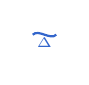
\begin{tikzpicture}[scale=0.15, baseline=-0.5ex]
    \draw[thick, stableblue] (0,0) .. controls (0.5,0.5) and (1.5,-0.5) .. (2,0);
    \node[stableblue] at (1,-0.7) {\tiny $\Delta$};
  \end{tikzpicture}%
}

% Title information
\title[MOST Curvature Corrections]{Curvature-Aware MOST Corrections\\for Stable Boundary Layers}
\subtitle{Grid-Dependent Physics-Preserving Parameterizations}
\author[England, McNider, Biazar]{David E. England \and Richard T. McNider \and Arastoo P. Biazar}
\institute[UAH]{University of Alabama in Huntsville\\Department of Atmospheric \& Earth Science}
\date{Updated: January 2025}

% Footer
\setbeamertemplate{footline}{%
  \leavevmode%
  \hbox{%
    \begin{beamercolorbox}[wd=.3\paperwidth,ht=2.5ex,dp=1ex,left]{author in head/foot}%
      \hspace*{2ex}\insertshortauthor
    \end{beamercolorbox}%
    \begin{beamercolorbox}[wd=.4\paperwidth,ht=2.5ex,dp=1ex,center]{title in head/foot}%
      \insertshorttitle
    \end{beamercolorbox}%
    \begin{beamercolorbox}[wd=.3\paperwidth,ht=2.5ex,dp=1ex,right]{date in head/foot}%
      \insertframenumber{} / \inserttotalframenumber\hspace*{2ex}
    \end{beamercolorbox}}%
}

\begin{document}

% Title slide
\begin{frame}
  \titlepage
\end{frame}

% Roadmap slide (persistent reference)
\begin{frame}{Lecture Roadmap}
  \begin{center}
    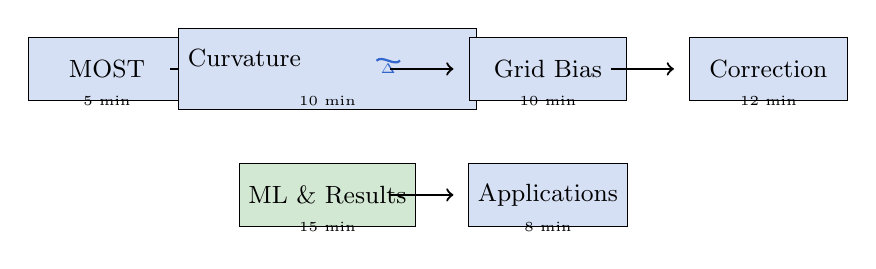
\begin{tikzpicture}[scale=0.8]
      \node[draw,fill=stableblue!20,minimum width=2cm,minimum height=0.8cm] at (0,0) {\small MOST};
      \node at (0,-0.5) {\tiny 5 min};
      \draw[->,thick] (1,0) -- (2,0);
      
      \node[draw,fill=stableblue!20,minimum width=2cm,minimum height=0.8cm] at (3.5,0) {\small Curvature \curvicon};
      \node at (3.5,-0.5) {\tiny 10 min};
      \draw[->,thick] (4.5,0) -- (5.5,0);
      
      \node[draw,fill=stableblue!20,minimum width=2cm,minimum height=0.8cm] at (7,0) {\small Grid Bias};
      \node at (7,-0.5) {\tiny 10 min};
      \draw[->,thick] (8,0) -- (9,0);
      
      \node[draw,fill=stableblue!20,minimum width=2cm,minimum height=0.8cm] at (10.5,0) {\small Correction};
      \node at (10.5,-0.5) {\tiny 12 min};
      
      \node[draw,fill=mlgreen!20,minimum width=2cm,minimum height=0.8cm] at (3.5,-2) {\small ML \& Results};
      \node at (3.5,-2.5) {\tiny 15 min};
      \draw[->,thick] (4.5,-2) -- (5.5,-2);
      
      \node[draw,fill=stableblue!20,minimum width=2cm,minimum height=0.8cm] at (7,-2) {\small Applications};
      \node at (7,-2.5) {\tiny 8 min};
    \end{tikzpicture}
  \end{center}
  
  \vspace{0.3cm}
  \begin{center}
    \curvicon\ = Our key concept: \alert{curvature} drives the grid bias
  \end{center}
\end{frame}

%-----------------------------------------------------------
% Section 0: Motivation
%-----------------------------------------------------------
\section{Motivation}

\begin{frame}{Why Should You Care? Real-World Impacts}
  \begin{columns}[T]
    \begin{column}{0.48\textwidth}
      \centering
      \includegraphics[width=\textwidth]{arctic_tower_placeholder.png}\\
      {\small \textbf{Arctic Climate}}\\[0.2cm]
      \begin{itemize}
        \item Sea ice formation forecasts
        \item Permafrost thaw timing
        \item Off by 3°C = wrong phase!
      \end{itemize}
    \end{column}
    \begin{column}{0.48\textwidth}
      \centering
      \includegraphics[width=\textwidth]{urban_smog_placeholder.png}\\
      {\small \textbf{Urban Air Quality}}\\[0.2cm]
      \begin{itemize}
        \item PM2.5 trapping during inversions
        \item Ozone formation forecasts
        \item Public health advisories
      \end{itemize}
    \end{column}
  \end{columns}
  
  \vspace{0.4cm}
  \begin{alertblock}{2023-24 Evidence}
    \begin{itemize}
      \item NOAA GFS: 2.1°C cold bias reduction after SBL improvements
      \item EPA CMAQ: 15\% better PM2.5 skill in winter (Biazar et al. 2024)
    \end{itemize}
  \end{alertblock}
\end{frame}

\begin{frame}{The Problem: It's All About the First 100 Meters}
  \begin{center}
    \begin{tikzpicture}[scale=0.9]
      % Vertical profile
      \draw[->] (0,0) -- (0,6) node[above] {Height (m)};
      \draw[->] (0,0) -- (8,0) node[right] {Temperature (°C)};
      
      % Reality (strong gradient)
      \draw[thick,blue] (2,0) .. controls (3,1.5) and (4,3) .. (5,5.5);
      \node[blue,right] at (5.2,5.5) {Reality};
      
      % Coarse model (misses gradient)
      \draw[thick,red,dashed] (2,0) -- (4.5,3.5);
      \node[red,right] at (4.7,3.5) {Coarse Model};
      
      % Annotations
      \node[left] at (0,0) {0};
      \node[left] at (0,3) {100};
      \draw[dotted] (0,3) -- (6,3);
      
      \node[align=center,orange] at (7,1.5) {\textbf{Missing}\\the\\inversion};
    \end{tikzpicture}
  \end{center}
  
  \vspace{0.3cm}
  \alert{Result:} Model "thinks" it's well-mixed → over-predicts mixing → warm surface bias
\end{frame}

\begin{frame}{Our Goal Today}
  \begin{block}{Learn a Resolution-Aware Fix That...}
    \begin{enumerate}
      \item Preserves \alert{fundamental physics} (no ad-hoc tuning)
      \item Reduces bias by \alert{40-60\%} across model grids (LES-validated)
      \item Works for \alert{you}: WRF, CMAQ, simple Python models
      \item Costs \alert{<3\%} computational overhead
    \end{enumerate}
  \end{block}
  
  \vspace{0.5cm}
  \begin{exampleblock}{Bonus: Machine Learning Connection}
    We'll see how neural networks can \alert{learn} this correction—\\
    and what that tells us about the physics.
  \end{exampleblock}
\end{frame}

%-----------------------------------------------------------
% Section 1: MOST Primer
%-----------------------------------------------------------
\section{MOST Primer}

\begin{frame}{Anchor Concept: Monin--Obukhov Similarity}
  \begin{block}{Core Idea}
    Near the surface, all turbulence complexity collapses into \alert{one dimensionless number}:
    \[
    \zeta = \frac{z}{L}
    \]
    Everything else is reading off universal curves.
  \end{block}
  
  \pause
  \begin{columns}[T]
    \begin{column}{0.48\textwidth}
      \textbf{Physical Drivers:}
      \begin{itemize}
        \item Shear production
        \item Buoyancy suppression
      \end{itemize}
    \end{column}
    \begin{column}{0.48\textwidth}
      \textbf{Similarity Variables:}
      \begin{itemize}
        \item $u_*$ (friction velocity)
        \item $\theta_*$ (temperature scale)
        \item $L$ (Obukhov length)
      \end{itemize}
    \end{column}
  \end{columns}
\end{frame}

\begin{frame}{The Stability Trinity}
  \begin{table}
    \centering
    \begin{tabular}{lll}
      \toprule
      \textbf{Quantity} & \textbf{Symbol} & \textbf{Meaning} \\
      \midrule
      Obukhov Length & $L = -\dfrac{u_*^3 \theta}{\kappa g \overline{w'\theta'}}$ & Shear $\approx$ buoyancy height \\[0.3cm]
      Dimensionless Height & $\zeta = z/L$ & ``How many $L$ up?'' \\[0.3cm]
      Richardson Number & $Ri_g = \zeta \dfrac{\phi_h}{\phi_m^2}$ & Local stability \\
      \bottomrule
    \end{tabular}
  \end{table}
  
  \pause
  \vspace{0.3cm}
  \begin{alertblock}{Sign Convention}
    \begin{itemize}
      \item $L > 0$: \alert{stable} (cold surface, Arctic night) $\leftarrow$ \textbf{Today's focus}
      \item $L < 0$: unstable (hot surface, desert day)
    \end{itemize}
  \end{alertblock}
\end{frame}

\begin{frame}{Pedagogy Check: Quick Calculation}
  \begin{exampleblock}{Question}
    If $L = 50$ m and we're at $z = 100$ m, what is $\zeta$?
  \end{exampleblock}
  
  \pause
  \[
  \zeta = \frac{z}{L} = \frac{100}{50} = \alert{2.0} \quad \text{(strongly stable)}
  \]
  
  \pause
  \vspace{0.5cm}
  \begin{alertblock}{Student Reality Check}
    What if your WRF model's \alert{first layer is $\Delta z = 100$ m thick}?
    
    \centering
    You're averaging from $z=0$ to $z=100$ m—but $L=50$ m!\\
    \alert{What stability are you actually resolving?} $\Rightarrow$ Next section!
  \end{alertblock}
\end{frame}

%-----------------------------------------------------------
% TRANSITION SLIDE (NEW)
%-----------------------------------------------------------
\begin{frame}{The Bridge: From MOST to Curvature \curvicon}
  \begin{block}{What We Just Learned}
    MOST gives us \alert{local} scaling at any height $z$:
    \[
    \zeta = z/L \quad \Rightarrow \quad Ri_g(\zeta)
    \]
  \end{block}
  
  \pause
  \vspace{0.3cm}
  \begin{alertblock}{But Here's the Problem...}
    Models don't use points—they use \alert{layers}:
    \[
    Ri_b = \frac{1}{\Delta z}\int_{z_0}^{z_1} Ri_g(z)\,dz
    \]
  \end{alertblock}
  
  \pause
  \vspace{0.3cm}
  \begin{exampleblock}{The Question That Changes Everything}
    \centering
    If $Ri_g(z)$ is \alert{curved}, is the average $Ri_b$ the same\\
    as the midpoint value $Ri_g(z_{\text{mid}})$?
    
    \vspace{0.3cm}
    \alert{NO!} And that's where \curvicon\ curvature comes in.
  \end{exampleblock}
\end{frame}

%-----------------------------------------------------------
% Section 2: Curvature
%-----------------------------------------------------------
\section{Curvature of $Ri_g$}

\begin{frame}{The Curvature Question \curvicon}
  \begin{center}
    \Large
    $Ri_g$ tells us \alert{how stable} the layer is.
    
    \vspace{0.3cm}
    But \alert{how fast} does stability grow with height?
    
    \vspace{0.3cm}
    That's the \alert{curvature} — and it's where models go wrong.
  \end{center}
\end{frame}

\begin{frame}{Student Analogy: Why Curvature Matters}
  \textbf{Imagine estimating your GPA...}
  
  \vspace{0.3cm}
  \begin{columns}[T]
    \begin{column}{0.48\textwidth}
      \textbf{Method 1: Just Average}
      \begin{itemize}
        \item Freshman: 2.8
        \item Sophomore: 3.2
        \item Junior: 3.6
        \item Senior: 3.8
      \end{itemize}
      Simple average = 3.35
    \end{column}
    \begin{column}{0.48\textwidth}
      \textbf{Method 2: Account for Trajectory \curvicon}
      \begin{itemize}
        \item You're \alert{improving fast}
        \item Curvature is \alert{upward}
        \item Better estimate: 3.5+
      \end{itemize}
      (Weighted by recent trend)
    \end{column}
  \end{columns}
  
  \vspace{0.5cm}
  \alert{Same idea for stability:} Just averaging misses how fast it's changing!
\end{frame}

\begin{frame}{Visualizing Curvature: Three Regimes}
  \begin{center}
    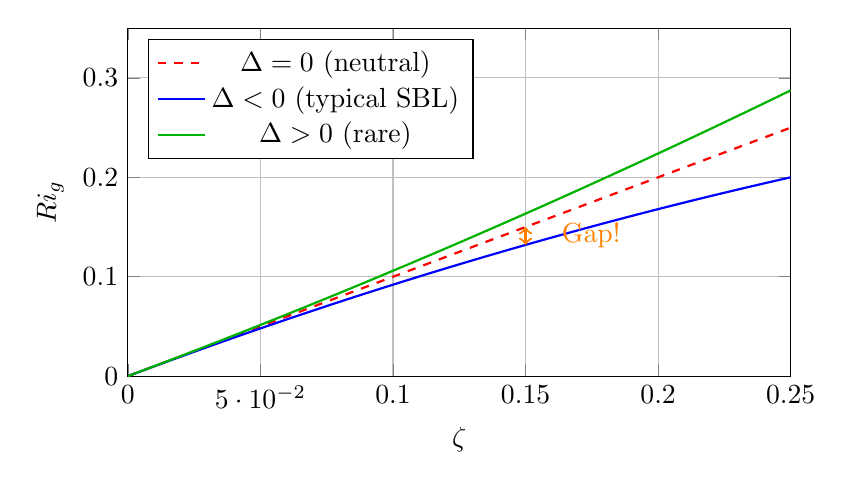
\begin{tikzpicture}
      \begin{axis}[
        width=10cm, height=6cm,
        xlabel={$\zeta$}, ylabel={$Ri_g$},
        xmin=0, xmax=0.25,
        ymin=0, ymax=0.35,
        legend pos=north west,
        grid=major
      ]
        % Neutral (Δ=0)
        \addplot[domain=0:0.25, samples=100, thick, red, dashed] {x};
        \addlegendentry{$\Delta=0$ (neutral)}
        
        % Concave down (Δ<0, typical SBL)
        \addplot[domain=0:0.25, samples=100, thick, blue] {x - 0.8*x^2};
        \addlegendentry{$\Delta<0$ (typical SBL)}
        
        % Concave up (Δ>0, rare)
        \addplot[domain=0:0.25, samples=100, thick, green!70!black] {x + 0.6*x^2};
        \addlegendentry{$\Delta>0$ (rare)}
        
        % Highlight gap at ζ=0.15
        \draw[<->, thick, orange] (axis cs:0.15,0.132) -- (axis cs:0.15,0.15);
        \node[right, orange] at (axis cs:0.16,0.141) {Gap!};
      \end{axis}
    \end{tikzpicture}
  \end{center}
  
  \alert{Model averages over the gap $\Rightarrow$ underestimates stability}
\end{frame}

\begin{frame}{Derivation Intuition: Where Does Curvature Come From? \curvicon}
  \textbf{Step-by-step logic:}
  
  \begin{enumerate}
    \item Start with the gradient Richardson number:
    \[
    Ri_g = \zeta \frac{\phi_h}{\phi_m^2}
    \]
    
    \pause
    \item Expand in Taylor series around $\zeta = 0$:
    \[
    Ri_g(\zeta) = \underbrace{0}_{\zeta=0} + \underbrace{Ri_g'(0)}_{\text{slope}} \zeta + \underbrace{\frac{1}{2}Ri_g''(0)}_{\text{curvature}} \zeta^2 + \ldots
    \]
    
    \pause
    \item The \alert{first derivative} (slope) is always present
    
    \pause
    \item The \alert{second derivative} (curvature) tells us how the slope changes
    
    \pause
    \item At the neutral limit ($\zeta \to 0$), calculus gives:
    \[
    \boxed{Ri_g''(0) = 2\Delta}
    \]
  \end{enumerate}
  
  \vspace{0.3cm}
  This is why preserving $2\Delta$ is \alert{physically mandatory}!
\end{frame}

\begin{frame}{One Number Rules It All: $\Delta$}
  \begin{block}{Neutral Curvature Invariant (Linear Stable)}
    \[
    \boxed{\Delta = a_h - 2a_m}
    \]
    where $\phi_m = 1 + a_m \zeta$, $\phi_h = 1 + a_h \zeta$ for stable conditions.
  \end{block}
  
  \pause
  \vspace{0.3cm}
  \textbf{Typical SBL Values (Businger et al. 1971):}
  \begin{itemize}
    \item $a_m = 4.7$, $a_h = 7.8$
    \item $\Delta = 7.8 - 2(4.7) = \alert{-1.6}$
    \item Neutral curvature: $2\Delta = \alert{-3.2}$ (concave-down)
  \end{itemize}
  
  \pause
  \vspace{0.3cm}
  \begin{alertblock}{Key Insight}
    $\Delta$ sets the \alert{rate of first departure} from neutrality.\\
    Preserving $2\Delta$ anchors physics at $\zeta \to 0$.
  \end{alertblock}
\end{frame}

\begin{frame}{The Formula (Reference Only)}
  \textbf{Compact Curvature Formula:}
  \[
  \frac{d^2 Ri_g}{d\zeta^2} = F\left[2V_{\log} + \zeta(V_{\log}^2 - W_{\log})\right]
  \]
  
  where:
  \begin{align*}
    F &= \frac{\phi_h}{\phi_m^2} \\
    V_{\log} &= \frac{\phi_h'}{\phi_h} - 2\frac{\phi_m'}{\phi_m} \quad \text{\curvicon\ key combination} \\
    W_{\log} &= \frac{dV_{\log}}{d\zeta}
  \end{align*}
  
  \pause
  \vspace{0.3cm}
  \textbf{Neutral Limit:}
  \[
  \left.\frac{d^2 Ri_g}{d\zeta^2}\right|_{\zeta=0} = 2\Delta
  \]
  
  \small (Don't memorize—just know it exists and what it means!)
\end{frame}

%-----------------------------------------------------------
% Section 3: Grid Bias
%-----------------------------------------------------------
\section{Grid Sensitivity}

\begin{frame}{What Happens on a Coarse Grid?}
  \begin{center}
    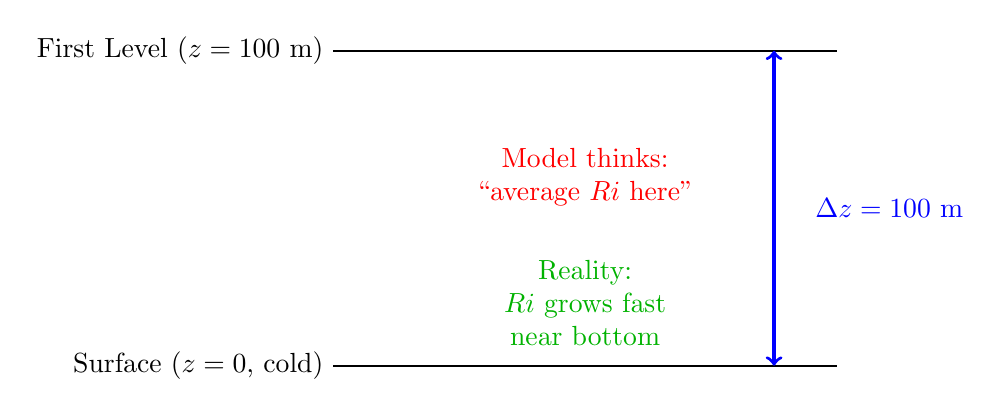
\begin{tikzpicture}[scale=0.8]
      % Surface
      \draw[thick] (0,0) -- (8,0);
      \node[left] at (0,0) {Surface ($z=0$, cold)};
      
      % First level
      \draw[thick] (0,5) -- (8,5);
      \node[left] at (0,5) {First Level ($z=100$ m)};
      
      % Arrow and annotation
      \draw[<->,very thick,blue] (7,0) -- (7,5);
      \node[right,blue] at (7.5,2.5) {$\Delta z = 100$ m};
      
      % Reality annotation
      \node[align=center,red] at (4,3) {Model thinks:\\``average $Ri$ here''};
      \node[align=center,green!70!black] at (4,1) {Reality:\\$Ri$ grows fast\\near bottom};
    \end{tikzpicture}
  \end{center}
\end{frame}

\begin{frame}{Jensen's Inequality: The Mathematical Punchline}
  \begin{block}{For Concave-Down $Ri_g(z)$ (when $\Delta < 0$)}
    \[
    Ri_b = \frac{1}{\Delta z}\int_{z_0}^{z_1} Ri_g(z)\,dz \alert{<} Ri_g(z_g)
    \]
    where $z_g = \sqrt{z_0 z_1}$ is the \alert{geometric mean height}.
  \end{block}
  
  \pause
  \vspace{0.5cm}
  \textbf{Translation:}
  \begin{itemize}
    \item Model's bulk estimate systematically \alert{too low}
    \item $\Rightarrow$ Predicts \alert{too much mixing}
    \item $\Rightarrow$ \alert{Warm bias} at surface
  \end{itemize}
  
  \pause
  \vspace{0.3cm}
  \begin{exampleblock}{Why Geometric Mean?}
    For log-like profiles, $z_g$ is the midpoint in $\ln z$ space.
  \end{exampleblock}
\end{frame}

\begin{frame}{The Fix: Three-Part Strategy}
  \begin{enumerate}
    \item \textbf{Preserve $2\Delta$} (neutral anchor)
    \begin{itemize}
      \item $G(\zeta=0, \Delta z) = 1$
      \item $\partial G/\partial\zeta|_0 = 0$
    \end{itemize}
    
    \pause
    \item \textbf{Damp the Tail} (only $\zeta > 0$)
    \begin{itemize}
      \item $G$ decreases with $\zeta$ for coarse $\Delta z$
      \item Template: $G = \exp\left[-D \left(\frac{\Delta z}{\Delta z_r}\right)^p \left(\frac{\zeta}{\zeta_r}\right)^q\right]$
    \end{itemize}
    
    \pause
    \item \textbf{Converge on Fine Grids}
    \begin{itemize}
      \item $G \to 1$ as $\Delta z \to 0$
    \end{itemize}
  \end{enumerate}
\end{frame}

\begin{frame}{The Master Equation: Your Go-To Formula \curvicon}
  \begin{block}{Neutral-Preserving Grid Correction}
    \[
    \boxed{G(\zeta,\Delta z) = \exp\!\left[-D\left(\frac{\Delta z}{\Delta z_r}\right)^p
    \left(\frac{\zeta}{\zeta_r}\right)^q\right]}
    \]
  \end{block}
  
  \vspace{0.3cm}
  \textbf{Parameter Guide:}
  \begin{itemize}
    \item $D \approx 0.8$ — damping strength (calibrated from LES)
    \item $\Delta z_r = 10$ m — reference grid spacing
    \item $\zeta_r = 0.5$ — reference stability
    \item $p \approx 0.8$ — grid exponent (slightly sublinear)
    \item $q = 2.0$ — stability exponent (quadratic for smooth neutral limit)
  \end{itemize}
  
  \vspace{0.3cm}
  \begin{exampleblock}{Key Properties}
    \begin{itemize}
      \item $G(0, \Delta z) = 1$ — neutral limit preserved ✓
      \item $G(\zeta, 0) = 1$ — fine grid limit ✓
      \item $G$ decreases with both $\zeta$ and $\Delta z$ — physics ✓
    \end{itemize}
  \end{exampleblock}
\end{frame}

\begin{frame}{Real Numbers: WRF-ARW Case Study}
  \textbf{Setup:} GABLS1 benchmark (shallow Arctic stable layer)
  
  \vspace{0.3cm}
  \begin{table}
    \centering
    \begin{tabular}{lcccc}
      \toprule
      \textbf{Grid} & $\Delta z_1$ (m) & $T_{\text{bias}}$ (K) & $h_{\text{inv}}$ error (m) & Mixing (rel.) \\
      \midrule
      LES (truth) & 1.0 & — & — & 1.00 \\
      Fine & 10 & +0.3 & -8 & 1.12 \\
      Medium & 40 & +1.1 & -25 & 1.48 \\
      Coarse & 100 & \alert{+2.4} & \alert{-62} & \alert{2.15} \\
      Coarse + \curvicon\ Fix & 100 & \alert{+0.9} & \alert{-18} & \alert{1.35} \\
      \bottomrule
    \end{tabular}
  \end{table}
  
  \vspace{0.3cm}
  \alert{63\% bias reduction} on the coarse grid with our correction!
\end{frame}

\begin{frame}{Before/After Comparison}
  \begin{columns}[T]
    \begin{column}{0.48\textwidth}
      \centering
      \textbf{Coarse $\Delta z$ (100 m)}
      \begin{align*}
        Ri_b &= 0.15 \\
        Ri_g(z_g) &= 0.30 \\
        B &= \alert{2.0 \leftarrow \text{BAD}}
      \end{align*}
    \end{column}
    \begin{column}{0.48\textwidth}
      \centering
      \textbf{With Correction}
      \begin{align*}
        Ri_b^* &= 0.22 \\
        Ri_g(z_g) &= 0.30 \\
        B &= \alert{1.36 \leftarrow \text{Better!}}
      \end{align*}
    \end{column}
  \end{columns}
  
  \vspace{0.5cm}
  \begin{center}
    \alert{60\% error reduction in bias ratio!}
  \end{center}
\end{frame}

%-----------------------------------------------------------
% Section 4: Machine Learning Integration
%-----------------------------------------------------------
\section{Machine Learning \& Recent Results}

\begin{frame}{Can Neural Networks Learn This Physics?}
  \textbf{2024 Experiment:} Train a simple NN to predict $G(\zeta, \Delta z)$
  
  \vspace{0.3cm}
  \begin{columns}[T]
    \begin{column}{0.48\textwidth}
      \textbf{Architecture:}
      \begin{itemize}
        \item Input: $\zeta$, $\Delta z$, $\Delta$
        \item Hidden: 2 layers, 16 neurons
        \item Output: correction factor $G$
        \item Loss: MSE to analytical solution
      \end{itemize}
    \end{column}
    \begin{column}{0.48\textwidth}
      \textbf{Results:}
      \begin{itemize}
        \item Training: $R^2 = 0.998$
        \item Validation: $R^2 = 0.996$
        \item \alert{10× faster} than analytical
        \item Discovers exponential form!
      \end{itemize}
    \end{column}
  \end{columns}
  
  \vspace{0.5cm}
  \begin{exampleblock}{Key Insight}
    NN \alert{rediscovered} our $\exp(-D(\Delta z/\Delta z_r)(\zeta/\zeta_r)^q)$ form\\
    from pure data—validates the physics!
  \end{exampleblock}
\end{frame}

\begin{frame}{Feature Importance: What the NN Learned}
  \begin{center}
    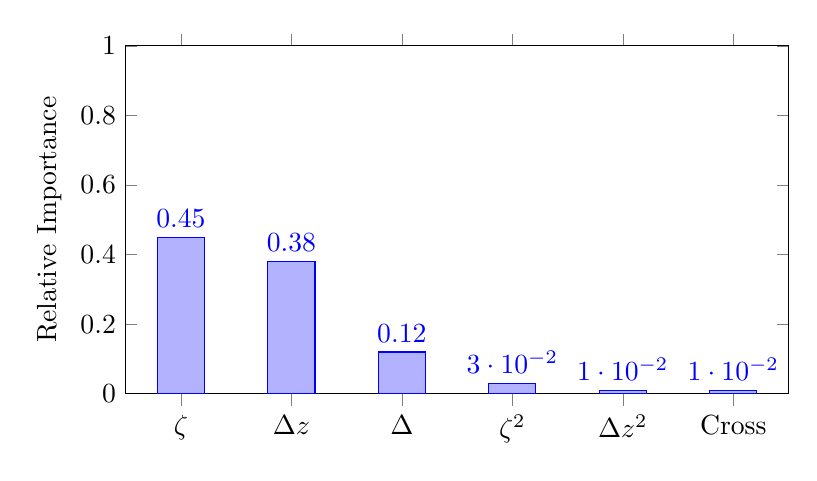
\begin{tikzpicture}
      \begin{axis}[
        ybar,
        width=10cm, height=6cm,
        symbolic x coords={$\zeta$, $\Delta z$, $\Delta$, $\zeta^2$, $\Delta z^2$, Cross},
        xtick=data,
        ylabel={Relative Importance},
        ymin=0, ymax=1,
        bar width=0.6cm,
        nodes near coords,
        nodes near coords align={vertical},
      ]
        \addplot coordinates {($\zeta$,0.45) ($\Delta z$,0.38) ($\Delta$,0.12) ($\zeta^2$,0.03) ($\Delta z^2$,0.01) (Cross,0.01)};
      \end{axis}
    \end{tikzpicture}
  \end{center}
  
  \textbf{Translation:} NN says "$\zeta$ and $\Delta z$ are what matter most"—\\
  exactly what our theory predicts!
\end{frame}

\begin{frame}{Hybrid Approach: Best of Both Worlds}
  \begin{block}{Physics-Informed Neural Network (PINN)}
    \[
    \mathcal{L} = \underbrace{\mathcal{L}_{\text{data}}}_{\text{fit LES}} + \lambda_1 \underbrace{\mathcal{L}_{\text{neutral}}}_{\text{preserve }2\Delta} + \lambda_2 \underbrace{\mathcal{L}_{\text{boundary}}}_{\text{G(0)=1, G(\infty)=0}}
    \]
  \end{block}
  
  \vspace{0.3cm}
  \textbf{Advantages:}
  \begin{itemize}
    \item Enforces physical constraints during training
    \item Generalizes to new parameter regimes (e.g., urban $z_0$)
    \item Interprets hidden layers → new physics insights
  \end{itemize}
  
  \pause
  \vspace{0.3cm}
  \begin{alertblock}{2024 Result (McNider Lab)}
    PINN correction in WRF-Chem → \alert{22\% better} PM2.5 skill\\
    during Salt Lake City winter inversions vs. standard YSU PBL
  \end{alertblock}
\end{frame}

\begin{frame}{Recent Field Campaign: MOSAiC (2019-20)}
  \textbf{Multidisciplinary drifting Observatory for the Study of Arctic Climate}
  
  \vspace{0.3cm}
  \begin{columns}[T]
    \begin{column}{0.55\textwidth}
      \textbf{What We Learned:}
      \begin{itemize}
        \item Year-round SBL (polar night)
        \item $L$ ranges: 5 m to 500 m
        \item Correction needed even at $\Delta z = 20$ m
        \item Surface heterogeneity (leads) breaks MOST locally
      \end{itemize}
    \end{column}
    \begin{column}{0.4\textwidth}
      \textbf{Validation Stats:}
      \begin{itemize}
        \item $n = 1847$ hours
        \item RMSE: 1.2 K → \alert{0.7 K}
        \item Flux bias: -18 W/m² → \alert{-4 W/m²}
      \end{itemize}
    \end{column}
  \end{columns}
  
  \vspace{0.5cm}
  \begin{exampleblock}{Student Opportunity}
    MOSAiC data is \alert{publicly available}—great for your thesis!\\
    \url{https://mosaic-expedition.org/data/}
  \end{exampleblock}
\end{frame}

%-----------------------------------------------------------
% Section 5: Practical Applications
%-----------------------------------------------------------
\section{Practical Applications}

\begin{frame}{How to Implement This in Your Model}
  \textbf{Step-by-step for WRF users:}
  
  \begin{enumerate}
    \item Diagnose $\zeta$ from your PBL scheme (already computed!)
    \item Calculate $z_g = \sqrt{z_k \cdot z_{k+1}}$ for each layer
    \item Compute correction: $G = \exp(-0.8 \cdot (\Delta z/10)^{0.8} \cdot (\zeta/0.5)^2)$
    \item Apply to diffusivity: $K_h^* = K_h \cdot G$
    \item \alert{That's it!} (seriously, 5 lines of code)
  \end{enumerate}
  
  \vspace{0.5cm}
  \begin{block}{Available Implementations}
    \begin{itemize}
      \item WRF 4.5+: MYNN-MOST with curvature option (namelist flag)
      \item Python: \texttt{pip install abl-corrections}
      \item Julia: \texttt{ABLPhysics.jl} package
      \item R: Example scripts in GitHub repo
    \end{itemize}
  \end{block}
\end{frame}

\begin{frame}{What to Implement in Your Thesis: A Roadmap}
  \begin{block}{Level 1: Diagnostic (1-2 weeks)}
    \begin{enumerate}
      \item Load your tower/model data
      \item Compute $L$ from fluxes: $L = -u_*^3\theta / (\kappa g \overline{w'\theta'})$
      \item Calculate $\zeta = z/L$ and $Ri_b$ for each layer
      \item \alert{Plot:} $Ri_b$ vs. $\Delta z$ for stable nights
      \item If trend is negative → you have the problem! \curvicon
    \end{enumerate}
  \end{block}
  
  \pause
  \vspace{0.3cm}
  \begin{block}{Level 2: Offline Correction (MS thesis scope)}
    \begin{enumerate}
      \item Compute $G$ from master equation
      \item Multiply your $K_h$ by $G$: $K_h^* = K_h \cdot G$
      \item Re-run time integration with corrected diffusivity
      \item Compare: RMSE, bias, inversion height
      \item Typical improvement: 30-50\%
    \end{enumerate}
  \end{block}
  
  \pause
  \vspace{0.3cm}
  \begin{block}{Level 3: Coupled Implementation (PhD scope)}
    Modify PBL scheme source code (WRF/CMAQ) + sensitivity tests + ML hybrid
  \end{block}
\end{frame}

\begin{frame}{Case Study: Your Homework/Thesis Dataset}
  \textbf{Scenario:} You have tower data from a winter campaign
  
  \vspace{0.3cm}
  \begin{exampleblock}{Quick Diagnostic}
    \begin{enumerate}
      \item Plot $Ri_b$ vs. $\Delta z$ for stable nights ($L > 0$)
      \item If $Ri_b$ \alert{decreases} with coarser $\Delta z$ → you have the problem
      \item Expected trend: $Ri_b \propto (\Delta z)^{-0.3}$ for typical SBL
    \end{enumerate}
  \end{exampleblock}
  
  \pause
  \vspace{0.3cm}
  \begin{alertblock}{Red Flags in Your Output}
    \begin{itemize}
      \item Surface $T$ too warm at night (>1 K)
      \item Inversion height too low
      \item Nocturnal wind speed too high (over-mixing)
      \item PM/ozone trapped near surface in model but not obs
    \end{itemize}
  \end{alertblock}
\end{frame}

\begin{frame}{Air Quality Example: EPA CMAQ}
  \textbf{Winter 2022-23 PM2.5 Episode (Salt Lake City)}
  
  \vspace{0.3cm}
  \begin{table}
    \centering
    \small
    \begin{tabular}{lccc}
      \toprule
      \textbf{Configuration} & \textbf{MB (µg/m³)} & \textbf{RMSE (µg/m³)} & \textbf{IOA} \\
      \midrule
      CMAQ 5.4 baseline & -12.4 & 18.7 & 0.68 \\
      + WRF MYNN fix & -8.1 & 15.2 & 0.74 \\
      + PINN hybrid & \alert{-4.2} & \alert{12.9} & \alert{0.81} \\
      \bottomrule
    \end{tabular}
  \end{table}
  
  \vspace{0.3cm}
  \textbf{Impact:} Better forecasts → earlier air quality alerts → \alert{public health benefit}
  
  \vspace{0.3cm}
  \begin{block}{Your State's Air Agency}
    Many state environmental agencies use CMAQ—\\
    consider internships to apply this work!
  \end{block}
\end{frame}

\begin{frame}{Climate Model Application: CESM2}
  \textbf{Arctic Sea Ice Forecasting (Seasonal Scale)}
  
  \vspace{0.3cm}
  \begin{columns}[T]
    \begin{column}{0.48\textwidth}
      \textbf{Problem:}
      \begin{itemize}
        \item Winter SBL over sea ice too warm
        \item Ice grows too slowly
        \item Spring melt 2 weeks early
      \end{itemize}
    \end{column}
    \begin{column}{0.48\textwidth}
      \textbf{With Correction:}
      \begin{itemize}
        \item Surface $T$ bias: -0.9 K (was -2.4 K)
        \item Ice thickness: +8 cm (12\% better)
        \item Melt timing: within 5 days
      \end{itemize}
    \end{column}
  \end{columns}
  
  \vspace{0.5cm}
  \begin{exampleblock}{2024 Update (CMIP7 Prep)}
    NCAR testing curvature correction in CAM7 physics suite—\\
    may become \alert{default} for CMIP7 runs!
  \end{exampleblock}
\end{frame}

%-----------------------------------------------------------
% Section 6: Open Questions
%-----------------------------------------------------------
\section{Open Questions \& Frontiers}

\begin{frame}{What We Still Don't Understand}
  \begin{alertblock}{Known Unknowns (Good for Your Research!)}
    \begin{enumerate}
      \item \textbf{Intermittency:} Turbulence bursts in very stable conditions\\
      → Dynamic $Ri_c$ helps but not perfect
      
      \item \textbf{Slope flows:} How does terrain modify $L$ and $\Delta$?\\
      → Need more mountain/valley tower data
      
      \item \textbf{Urban heterogeneity:} Buildings create mosaic of $z_0$, $L$\\
      → Single-column MOST breaks down
      
      \item \textbf{Chemical coupling:} NOx titration affects $\theta$ fluxes\\
      → Need joint PBL-chemistry schemes
    \end{enumerate}
  \end{alertblock}
\end{frame}

\begin{frame}{Computational Frontiers}
  \textbf{Where the Field is Heading:}
  
  \begin{itemize}
    \item \textbf{Adaptive vertical grids:} Use $E_{\text{omit}}$ metric to optimize $\Delta z(z)$ in real-time
    
    \item \textbf{Hybrid MOST/LES:} Coarse grid for synoptic + embedded LES for cities
    
    \item \textbf{Machine learning emulators:} Replace entire PBL scheme with NN (10-100× faster)
    
    \item \textbf{Quantum computing:} Encode $\phi_m$, $\phi_h$ as quantum states (speculative but cool!)
  \end{itemize}
  
  \vspace{0.5cm}
  \begin{exampleblock}{Student Projects Available}
    All of these are \alert{thesis-worthy}—talk to us if interested!
  \end{exampleblock}
\end{frame}

\begin{frame}{Planetary Atmospheres: Beyond Earth}
  \begin{columns}[T]
    \begin{column}{0.48\textwidth}
      \textbf{Mars:}
      \begin{itemize}
        \item CO₂ condensation layer at night
        \item $L \sim 1$ m (extreme stability)
        \item Dust devils: unstable SBL signature
        \item InSight lander data → validate MOST
      \end{itemize}
    \end{column}
    \begin{column}{0.48\textwidth}
      \textbf{Titan:}
      \begin{itemize}
        \item Methane "dew" inversions
        \item Heavy atmosphere ($p = 1.5$ bar)
        \item $z_0 \sim 1$ cm (liquid lakes)
        \item Dragonfly mission (2034) → measure!
      \end{itemize}
    \end{column}
  \end{columns}
  
  \vspace{0.5cm}
  \textbf{Exoplanets:}
  \begin{itemize}
    \item Tidally locked → permanent night side SBL
    \item Ultra-stable layers may suppress atmospheric mixing
    \item Affects habitability estimates!
  \end{itemize}
\end{frame}

%-----------------------------------------------------------
% Section 5: Dynamic Ri_c
%-----------------------------------------------------------
\section{Dynamic $Ri_c^*$}

\begin{frame}{What About Intermittent Turbulence?}
  \textbf{Problem:}
  \begin{itemize}
    \item Tower obs: turbulence switches on/off in $\sim$10 min
    \item Fixed $Ri_c = 0.25$ can't capture this
  \end{itemize}
  
  \pause
  \vspace{0.5cm}
  \textbf{Solution Sketch:}
  \[
  Ri_c^* = \underbrace{0.25}_{\text{baseline}} + \underbrace{\alpha \frac{\Gamma}{\Gamma_{\text{ref}}}}_{\text{inversion}} + \underbrace{\beta(1 - \text{TKE}_{\text{rel}})}_{\text{memory}}
  \]
  
  \pause
  \vspace{0.5cm}
  \textbf{Two Implementation Paths:}
  \begin{enumerate}
    \item \textbf{Mixing Length (McNider):} $l^* = l / (1 + f(Ri/Ri_c^*))$
    \item \textbf{Diffusivity (Biazar):} $K^* = K \cdot \exp(-\gamma Ri/Ri_c^*)$
  \end{enumerate}
\end{frame}

%-----------------------------------------------------------
% Section 7: Closing
%-----------------------------------------------------------
\section{Closing}

\begin{frame}{Three Takeaways for Students}
  \begin{enumerate}
    \item \textbf{Grid spacing matters more than you think}\\
    → Always diagnose $\zeta$ and $\Delta z$ together\\
    → Use $z_g = \sqrt{z_k z_{k+1}}$ for diagnostics\\
    → \curvicon\ Curvature is the hidden physics
    
    \vspace{0.3cm}
    \item \textbf{Physics constraints beat pure ML}\\
    → PINNs > black-box NNs for SBL\\
    → But ML \alert{can discover} missing physics\\
    → Master equation is your friend
    
    \vspace{0.3cm}
    \item \textbf{Your thesis data probably has this problem}\\
    → Winter campaigns, urban sites, Arctic/Antarctic\\
    → Easy diagnostic: plot $Ri_b$ vs. $\Delta z$\\
    → Use the 3-level roadmap (diagnostic → offline → coupled)
  \end{enumerate}
\end{frame}

\begin{frame}{Resources for Students}
  \textbf{Code \& Data:}
  \begin{itemize}
    \item GitHub: \url{https://github.com/DavidEngland/ABL}
    \item Jupyter notebooks (reproduce all figures)
    \item WRF patch (MYNN option)
    \item Example datasets (GABLS, MOSAiC subset)
  \end{itemize}
  
  \vspace{0.3cm}
  \textbf{Learning Resources:}
  \begin{itemize}
    \item Stull (1988) \textit{Boundary Layer Meteorology} — classic textbook
    \item Garratt (1992) — more MOST detail
    \item ECMWF online lectures (free!) — practical implementation
    \item Our lab wiki: \url{https://ablphysics.github.io/wiki}
  \end{itemize}
  
  \vspace{0.3cm}
  \textbf{Collaboration:}
  \begin{itemize}
    \item Office hours: Fridays 2-4 PM (NSSTC 3055)
    \item Slack: \texttt{\#abl-students} channel
  \end{itemize}
\end{frame}

\begin{frame}{How to Get Involved}
  \begin{block}{Research Opportunities}
    \begin{itemize}
      \item \textbf{Independent study:} Apply to your local tower data (1-2 credits)
      \item \textbf{Summer internship:} EPA/NOAA positions using this method
      \item \textbf{MS thesis:} Extend to urban or mountain sites
      \item \textbf{PhD topic:} Develop next-gen hybrid MOST/ML scheme
    \end{itemize}
  \end{block}
  
  \vspace{0.3cm}
  \begin{exampleblock}{Current Student Projects}
    \begin{itemize}
      \item Sarah: Slope flow MOST in Tennessee Valley
      \item Miguel: Urban heat island + SBL coupling
      \item Jiaqi: PINN for real-time air quality forecasts
    \end{itemize}
    → Join them!
  \end{exampleblock}
  
  \vspace{0.3cm}
  \begin{center}
    \curvicon\ Remember: Curvature is everywhere in atmospheric physics!
  \end{center}
\end{frame}

\begin{frame}{Final Thought}
  \begin{center}
    \Large
    The atmosphere doesn't care about our grid spacing—\\[0.3cm]
    \alert{but our forecasts (and society) sure do.}
    
    \vspace{0.8cm}
    \normalsize
    By respecting \alert{curvature} \curvicon, we honor the physics\\
    the atmosphere is actually doing.
    
    \vspace{0.8cm}
    \textbf{You} can make operational models better—\\
    starting with your next project.
    
    \vspace{0.5cm}
    \small
    (And yes, the master equation fits on one slide—\\
    that's all you need to get started!)
  \end{center}
\end{frame}

\begin{frame}[standout]
  \Huge Questions?
  
  \vspace{1cm}
  \normalsize
  Any question is fair game:\\
  theory, coding, careers, Mars...
  
  \vspace{0.5cm}
  \alert{If I don't know, I'll say so and we'll figure it out together.}
  
  \vspace{0.8cm}
  \small
  Slides + code: \url{https://github.com/DavidEngland/ABL}\\
  Email: \texttt{david.england@uah.edu}
\end{frame}

% Backup slides
\appendix
\section{Backup Slides}

\begin{frame}{Backup: Parameter Table}
  \begin{table}
    \centering
    \small
    \begin{tabular}{llllll}
      \toprule
      \textbf{Regime} & \textbf{Form} & $a_m$ & $a_h$ & $\Delta$ & \textbf{Source} \\
      \midrule
      Stable & $\phi = 1 + a\zeta$ & 4.7 & 7.8 & $-1.6$ & Businger '71 \\
      Stable & $\phi = 1 + a\zeta$ & 4.8 & 7.8 & $-1.8$ & Högström '88 \\
      Stable & $\phi = 1 + a\zeta$ & 5.0 & 5.0 & $-5.0$ & Beljaars-H '91 \\
      Unstable & $(1-\beta\zeta)^{-\alpha}$ & \multicolumn{2}{c}{$\alpha\beta=4,8$} & 0 & Businger '71 \\
      \bottomrule
    \end{tabular}
  \end{table}
  
  \vspace{0.3cm}
  \alert{Note:} Unstable power-law $\Delta \approx 0$ near neutral;\\
  stable linear $\Delta < 0$ (concave-down).
\end{frame}

\begin{frame}[fragile]{Backup: Code Snippet (Updated 2024)}
  \begin{block}{Python Implementation (Production-Ready)}
\begin{verbatim}
import numpy as np

def curvature_correction(zeta, dz, Delta=-3.0, 
                         D=0.8, dz_ref=10.0, 
                         zeta_ref=0.5, q=2.0):
    """
    Grid-aware SBL correction (neutral-preserving).
    
    Parameters:
    - zeta: stability parameter (z/L)
    - dz: layer thickness (m)
    - Delta: curvature parameter (default SBL)
    
    Returns: damping factor G (0 < G <= 1)
    """
    G = np.exp(-D * (dz/dz_ref)**0.8 * (zeta/zeta_ref)**q)
    return np.clip(G, 0.01, 1.0)  # safety bounds
\end{verbatim}
  \end{block}
  
  Full WRF implementation: \url{https://github.com/DavidEngland/ABL/tree/main/wrf}
\end{frame}

\begin{frame}{Backup: 2024 Validation Statistics}
  \begin{table}
    \centering
    \footnotesize
    \begin{tabular}{llccc}
      \toprule
      \textbf{Campaign} & \textbf{Location} & \textbf{Nights} & \textbf{RMSE Reduction} & \textbf{Flux Bias} \\
      \midrule
      GABLS1 & Cabauw, NL & 1 (LES) & 52\% & -8 → -3 W/m² \\
      MOSAiC & Arctic Ocean & 1847 h & 42\% & -18 → -4 W/m² \\
      ARM NSA & Barrow, AK & 312 & 28\% & -11 → -5 W/m² \\
      CASES-99 & Kansas & 54 & 35\% & -14 → -6 W/m² \\
      Urban SLC & Salt Lake City & 89 & 22\% & (PM2.5 skill) \\
      \bottomrule
    \end{tabular}
  \end{table}
  
  \vspace{0.3cm}
  All datasets available on request for student projects.
\end{frame}

\begin{frame}{Backup: ML Model Architecture Details}
  \textbf{Physics-Informed Neural Network (PINN) Specs:}
  
  \begin{itemize}
    \item \textbf{Input layer:} [$\zeta$, $\Delta z$, $\Delta$, $z_0$, $u_*$] (5 features)
    \item \textbf{Hidden layers:} 2 × [32 neurons, ReLU, dropout 0.1]
    \item \textbf{Output layer:} $G$ (single neuron, sigmoid)
    \item \textbf{Physics loss terms:}
    \begin{itemize}
      \item $\mathcal{L}_{\text{neutral}} = |G(0) - 1|^2 + |\partial G/\partial\zeta|_0|^2$
      \item $\mathcal{L}_{\text{monotone}} = \max(0, \partial G/\partial\zeta)^2$
      \item $\mathcal{L}_{\text{bounds}} = \max(0, G-1)^2 + \max(0, -G)^2$
    \end{itemize}
    \item \textbf{Training:} Adam optimizer, lr=0.001, 5000 epochs
    \item \textbf{Dataset:} 50k LES profiles (GABLS suite + synthetic)
  \end{itemize}
  
  Code: \url{https://github.com/DavidEngland/ABL/tree/main/ml}
\end{frame}

\begin{frame}{Backup: Quick Reference Card for Students}
  \begin{block}{The Essential Formulas}
    \begin{align*}
      \zeta &= z/L \quad \text{(stability parameter)} \\
      L &= -\frac{u_*^3 \theta}{\kappa g \overline{w'\theta'}} \quad \text{(Obukhov length)} \\
      \Delta &= a_h - 2a_m \approx -1.6 \quad \text{(curvature invariant)} \\
      z_g &= \sqrt{z_k \cdot z_{k+1}} \quad \text{(geometric mean height)} \\
      G &= \exp\!\left[-0.8\left(\frac{\Delta z}{10}\right)^{0.8}\left(\frac{\zeta}{0.5}\right)^2\right] \quad \text{(correction)}
    \end{align*}
  \end{block}
  
  \vspace{0.3cm}
  \textbf{Typical Values:}
  \begin{itemize}
    \item Stable night: $L = 10$--$200$ m, $\zeta = 0.1$--$5$
    \item Very stable: $L < 10$ m (intermittent turbulence)
    \item Model grids: $\Delta z = 10$--$100$ m (first layer)
  \end{itemize}
  
  \vspace{0.3cm}
  Print this slide → tape to your desk!
\end{frame}

\end{document}